
\subsection{EXT4 文件系统的实现过程}

\subsubsection{LA 体系下 FAT32 与 EXT4 的区别}

\begin{enumerate}
    \item \textit{与指令集相关}
    % INPROCESS
    \item \textit{与 NPUcore 相关}
    % INPROCESS
\end{enumerate}

\subsubsection{敲定实现方式}

我们参考了历年不同赛道的优秀作品,最后给出了如下的适配方式:

\textit{我们采用第三方包将稳定 C 库作为外部库调入 NPUcore 中,如下图所示:}

\begin{table}[htbp]
    \centering
    \begin{tabular}{|c|c|}
        \hline
        选用技术栈 & 作用 \\
        \hline
        lwext4 & 稳定的 ext4 文件系统外部库 \\
        bindgen & rust-lang 官方开发的FFI生成工具 \\
        \hline
    \end{tabular}
    \caption{选用技术栈}
\end{table}

\newpage

\begin{figure}[htbp]
    \centering
    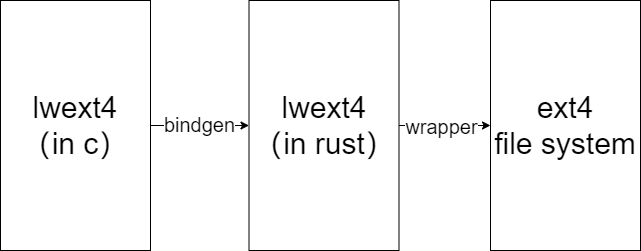
\includegraphics[width=0.6\linewidth]{figs/plan-ext.png}
    \caption{ext4 实现结构图}
    \label{ext4-complexe}
\end{figure}

\begin{enumerate}
    \item \textit{根据 lwext4 或者类似的库理清楚他的函数调用,必要的话给出一个 .h 文件用于包装函数入口:} \\ \textit{The wrapper.h file will include all the various headers containing declarations of structs and functions we would like bindings for. In the particular case of bzip2, this is pretty easy since the entire public API is contained in a single header. For a project like SpiderMonkey, where the public API is split across multiple header files and grouped by functionality, we'd want to include all those headers we want to bind to in this single wrapper.h entry point for bindgen.}\footnote{参考 bindgen 手册https://rust-lang.github.io/rust-bindgen/tutorial-2.html},这意味着,\textbf{对于一个比较复杂而分散的项目,我们最好给出一个包装文件}.
    \item \textit{对于转换完成的rs库,视情况给出rust调用}
    \item \textit{转换我们的fs适配新的rs库} \\ 这部分很简单,我们相当于已经拿来一个ext文件系统了,剩下的就是直接使用调用就行了。在makefile里和rust代码里加入feature就可以做到针对不同文件系统的编译与运行
\end{enumerate}

\subsubsection{第一次适配( LWEXT4-C + Bindgen )}

\subsubsection{第二次适配( LWEXT4-RUST )}

\subsubsection{第三次适配()}

\subsubsection{第四次适配()}